\documentclass[12pt]{article}
\usepackage[utf8]{inputenc}
\usepackage{mphysproject} % This includes graphicx, caption and geometry
\usepackage[block=space,bibencoding=utf8,style=phys,maxbibnames=6]{biblatex}
\usepackage{amsmath}
\usepackage{physics}
\usepackage{siunitx}

\usepackage{hyperref}
\usepackage{cleveref}
\usepackage{float}
\usepackage{stackengine}

\usepackage{lipsum}

\allowdisplaybreaks

\newcommand\textbff[1]{\textbf{\boldmath #1}}
\newcommand\circled[1]{\raisebox{.5pt}{\textcircled{\raisebox{-.9pt} {#1}}}
    }
\newcommand{\shortnote}[1]{\textit{\footnotesize (#1)}}

\newcommand{\pp}{\partial}
\newcommand{\mgrad}{\su{\nabla}}

% We often use underlines here
\stackMath
\newcommand\barbelow[1]{\stackunder[1.2pt]{#1}{\rule{1.5ex}{.1ex}}}
\newcommand{\su}[1]{\barbelow{#1}}
\newcommand{\du}[1]{\barbelow{\barbelow{#1}}}
\newcommand{\ssu}[1]{\scriptsize\barbelow{#1}\normalsize}
\newcommand{\sdu}[1]{\scriptsize\barbelow{\barbelow{#1}}\normalsize}

\newcommand{\NN}{$\su{N}$}
\newcommand{\EE}{$\du{E}$}
\newcommand{\PP}{$\du{\Pi}$}
\newcommand{\ddelta}[4]{\delta_{#1#3}\delta_{#2#4} + \delta_{#1#4}\delta_{#2#3}}

\newcommand{\onedot}{$\mathsurround0pt\ldotp$}
\newcommand{\cddot}{\mathbin{
    \vcenter{\baselineskip1ex \vspace{-0.1ex}\hbox{\onedot}\hbox{\onedot}}
}}

\begin{document}

\title{Normal Complex Tensor Order Parameter for Smectics in 3D}
\author{Jan Kocka}
\supervisor{Tyler N Shendruk}
%\date{1st January 2018}

\begin{abstract}
    \lipsum[10]
\end{abstract}

\maketitle

% This command introduces the Personal Statement: DO NOT REMOVE IT
\personalstatement
% Write PS here
\acknowledgments
% Write Acknowledgements here

\maintext

\section{Background}
\section{Smectic Liquid Crystals}
All physicists will be well familiar with the ordered crystalline phase, in which the relative positions and possibly orientation of molecules is ordered, predictable and often repeating.
Liquid crystals (LC) lay between this state and a typical liquid, some aspects of the phase are ordered, but others are not.
This is best illustrated as a transition from an unordered (isotropic) liquid state as in \cref{fig:phases}.

In an isotropic liquid the molecules have random, uncorrelated positions and orientations.
The first step in ordering is usually a transition to a polar or more commonly nematic liquid crystal in which the orientations of nearby molecules align (polar LC molecules have a head and tail, nematic are symmetric).
Next can come partial order in the positions of nearby molecules, this is the smectic phase.
There are many different types of smectic order, the simplest of which is layering as shown in \cref{fig:phases}.
In these layers there is positional order along the direction of layering as we can reliably predict there is likely to be molecules at the next layer and not in between them.
However, there is positional disorder in the other directions as we cannot predict molecular positions within the layers.

The simplest examples of such layering are smectic A and C phases which also have nematic order and in smectic A phases the directions of the two orders are aligned, whereas in smectic C phases they are at an angle (see \cref{fig:phases}).
There are many other smectic phases, smectic B have a hexagonal like structure, smectic E resembles C but the angle alternates between layers.
However, all exhibit some form of layering, that is what we focus on in this project.
In essence, we attempt to create a mesoscopic model that represents layering as such.
Such a model can then be coupled to others, say a one for nematic order, to represent the different types of smectics.

(Paragraph on why are they important/useful etc, obviously mention soap displays and hopefully something new? Bacteria! that might want a citation)

\begin{figure}
    \begin{center}
        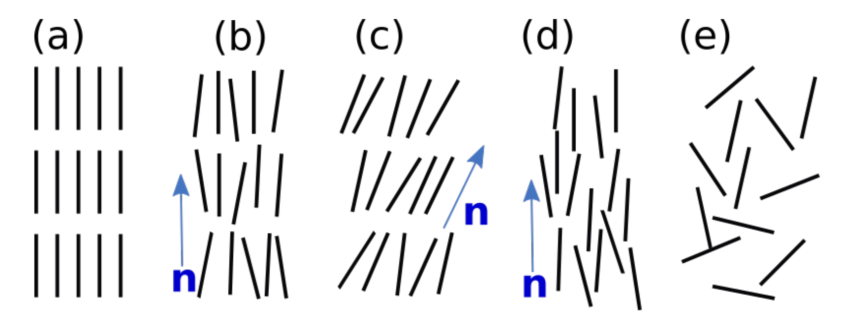
\includegraphics[width=0.95\textwidth]{figures/phases.pdf}
    \end{center}
    \caption{
        Illustrative structures of a substance made up from long molecules.
        In order from (a) to (e) they are a fully crystalized phase, a smectic A, smectic C, nematic and an isotropic liquid.
    }\label{fig:phases}
\end{figure}

\section{Rest of Background}
\subsection{Ginzburg-Landau theory intro?}
\subsection{Wirtinger derivatives (maybe move at the end?)}
\subsection{Describing smectics}
\subsection{Limitations we address and other approaches}

\section{Introduction to the \EE\ tensor}
We start by considering the density fluctuation as we have before
\begin{equation}
    \rho \simeq \rho_0 + 2\Re(\psi e^{i \ssu{q_0} \cdot \ssu{r}})
\end{equation}
but we allow the complex $\psi$ and the direction of $\su{q_0}$ both to be vary as fields leading to the wave part of the density being
\begin{equation}
    |\psi(\su{r})|e^{i (q_0 \ssu{N}(\ssu{r}) \cdot \ssu{r} + \phi(\ssu{r}))}
\end{equation}
with $q_0$ corresponding to the natural spacing of the wave.
Both $\su{N}$ and $\phi$ influence the phase, as before a constant gradient in $\phi$ corresponding to a constant contraction/dilation.


\section{New perspectives on \EE\ (in 3D)}
\subsection{Constraints}
\subsection{Biaxiality}
\subsection{Properties of biaxial \EE}
\begin{align}
    \du{E} &= \psi_1 (\su{N}\su{N} - \frac{\du{\delta}}{d}) + \psi_2 (\su{M}\su{M} - \frac{\du{\delta}}{d}) \\
    |\du{E}|^2 &= \du{E} \cddot \du{E}^* = (|\psi_1|^2 + |\psi_2|^2) (1 - 2 \frac{1}{d} + \frac{d}{d^2}) + (\psi_1\psi_2^* + \psi_1^*\psi_2) (-2\frac{1}{d} + \frac{d}{d^2}) \\
    &= \frac{d-1}{d} (|\psi_1|^2 + |\psi_2|^2) - \frac{1}{d} (\psi_1\psi_2^* + \psi_1^*\psi_2) \\
    &= (|\psi_1|^2 + |\psi_2|^2) - \frac{1}{d} (|\psi_1|^2 + |\psi_2|^2 + \psi_1\psi_2^* + \psi_1^*\psi_2) \\
    &= |\psi_1|^2 + |\psi_2|^2 - \frac{|\psi_1 + \psi_2|^2}{d} \\
    |\du{E_{eq}}|^2 &= \frac{d-1}{d}
\end{align}

\section{Dynamics of \EE}
\subsection{Ginzburg-Landau}
\subsection{Free Energy}
\subsubsection{Bulk}

\begin{align}
    f_\text{bulk} = A |\du{E}|^2 - \frac{C}{2}|\du{E}|^4 \rightarrow |\du{E_{eq}}|^2 = \frac{A}{C}
\end{align}

\section{Numerical Results}
\subsection{Imposed twist}
\subsubsection{Fitting $\frac{\theta}{\Delta\theta}$}
We now want to quantify the shapes of the azimuthal angle $\theta$ as a function of height.
To do that, we first of all non-dimensionalize these quantities and instead look at $\frac{\theta}{\Delta\theta}$ as a function of $\frac{h}{H}$.
That way all the plots will have the same end points and so can be compared, notably these endpoints will be at $(0, 0)$ and $(1, 1)$ and by symmetry they also ought to go through $(\frac{1}{2}, \frac{1}{2})$.
Further as the shape is clearly a sigmoidal one, we attempted a fit using both the $\arctan$ and the $\tanh$ functions, both of which only leave one parameter once the endpoints are fixed.
As the $\arctan$ method performed qualitatively better (see (CREF) for an example comparison of the two), we only use that from now on.
Its exact form is
\begin{equation}
    \frac{\theta}{\Delta\theta} = \frac{\arctan(a \qty(\frac{h}{H} - \frac{1}{2}))}{2\arctan(\frac{a}{2})} + \frac{1}{2}
\end{equation}
and we also quote that the slope of this function evaluated at $\frac{h}{H} = \frac{1}{2}$ is
\begin{equation}
    \eval{\dv{\frac{\theta}{\Delta\theta}}{\frac{h}{H}}}_\text{middle} = \frac{a}{2\arctan(\frac{a}{2})}
\end{equation}

\section{Current limitations of \EE}
\subsection{The smectic symmetries}
Earlier, in the motivational part of this thesis I have mentioned that one of the advantages of \EE\ is that it respects the symmetry of reversing the layering direction \NN\ both globally and locally.
While this is the true symmetry of a layered system, it is not a symmetry of the established relation between $|\psi|,\phi,\su{N}$ and the density modulation
\begin{equation}\label{eq:lim_den2}
    \rho(\su{r}) = \rho_0 + \Re(|\psi| e^{i(q_0\ssu{N}\cdot\ssu{r} + \phi)}), \qq{$|\psi|,\su{N}$ and $\phi$ being fields}
\end{equation}
which we did not directly use in this work, but it heavily guided our interpretation of the field.
The only symmetry of \cref{eq:lim_den2} is under simultaneously exchanging $\su{N}, \phi \leftrightarrow -\su{N}, -\phi$ locally or globally.
There are naturally two ways to resolve this issue.
Either modify \EE, in particular its complex phase, such that it respects the symmetry of \cref{eq:lim_den2}.
Or find a different way to interpret the fields from \EE\ as it is, or perhaps a combination of both approaches.

For modifying \EE, I suspect this would be very difficult to the point where any suitable form of \EE\ would likely be so different it should be called something else.
This is as one would need to somehow couple the complex phase $\phi$ and \NN, an eigenvector of \EE, which is only accessible numerically.
This is as the only symmetry of \cref{eq:lim_den2} is when the signs of both flip, not just one.
Regardless, if one was to find a form for \EE\ that satisfied both symmetries independently the interpretation of $\phi$ would not hold anymore.
Currently, using \cref{eq:lim_den2}, we interpret $\dv{\phi}{x}$ (with x being the direction along \NN\ at any point) as a contraction if it is positive and dilation if negative.
However, the change of $\phi \rightarrow -\phi$ will change the sign of these and so clearly this is not a physical symmetry of the system.

Thus, it seems the more natural way to move forward is to adapt \cref{eq:lim_den2} to respect the symmetry in \NN\ only.
Starting from a wave resembling $e^{i(\ssu{q_0}\cdot\ssu{r})}$ of which we want to adjust the wavelength locally.
Given the addition in \cref{eq:lim_den2} using $e^{i(\ssu{q_0}\cdot\ssu{r})(1+s(\ssu{r}))}$ might be a good starting point, where $s=0$ corresponds to equilibrium spacing, $s>1$ to a contraction and $s<1$ to a dilation.
This form has the required symmetry and can be expanded as
\begin{equation}
    e^{i(\ssu{q_0}\cdot\ssu{r})(1+s(\ssu{r}))} = e^{i(q_0\ssu{N}\cdot\ssu{r} + s(\ssu{r})q_0\ssu{N}\cdot\ssu{r})} 
\end{equation}
which now has the same form as \cref{eq:lim_den2} with $\phi(\su{r}) = s(\su{r})q_0\su{N}\cdot\su{r}$, however it is very important to stress that that would no longer be the $\phi$ from \EE\ as that would not change anything.
However, $s$ and $\phi$ from \EE\ are both dimensionless quantities and perhaps we can find a way to map them onto each other.
The only reasonable values for $s$ are from $-1$, where the wavelength becomes infinite, to $+\inf$ where wavelength goes to 0.
Any values $<-1$ would just correspond to a different $s$ and a flipped $\su{N}$.
On the other hand $\phi$ from \EE\ belongs to any set interval of length $2\pi$.
So if we use $\phi \in (-\pi, \pi]$ and let $s = \frac{\phi}{\pi}$ then the model could account for any dilation and a contraction of up to half the natural wavelength.
However, this would fundamentally change what $\phi$ from \EE\ is and would require more work to investigate any free energy costs to contractions and dilations, among other considerations.

\end{document}
